\Chapter{Storing plot state of a game world}

% 1. Define plot
\section{Definition of plot state}

All events happening within the game world form the plot of the game.
The way the plot is presented to the player depends on the narrative.
In other words the narrative is the plot with added context and presented using a certain storytelling technique.
The reception of the narrative by the player is often less dependent on the plot than it is on the technique used to present it.
In this thesis, the focus is not on the narrative but rather just the formal representation of the plot itself.
The plot consists of all events, characters and their actions in the game, all of which do not need to be available to the player or even exist in any way as separate beings.
Characters and their actions can be parts of the plot in the form of writing or recordings and events can be referenced in the history of the simulated world even though they were never really represented.
The actual form of the plot depends on the type of the game and the narrative it tries to establish.
As noted by Lindley, the plot state of the game world does not need to be available and presented to the player in its entirety, as is the case for example in games such as SIM City \cite{lindley2005story}.
In many games the player experiences a subset of the available plot and thus forms their own customized narrative.

Saussure introduced the distinction between language (la langue) and meaning (la parole)\cite{gordon2004langue}.
This distinction is similar to the difference between plot and narrative and likewise applicable in the context of plot representation alone.
In Saussure's framework, language (la langue) refers to the overall system of rules, conventions, and structures that govern a particular language, while meaning (la parole) refers to the individual utterances or expressions produced by speakers of that language.
This distinction emphasizes the idea that language is a system that is shared and agreed upon by a community of speakers, and that meaning is not fixed but rather is created through the interaction between the language system and the speaker's intentions and context.
When representing the plot state of a game world, it is important to consider the language used to describe that world and the range of expressions that are possible within that language.

Because it is impossible to consider the various approaches to formalize the representation of the game's plot without taking into account the constraints, limitations and requirements of the game in question, evaluation scenarios are defined in regards to which the described methods are evaluated.

% 2. Define evaluation scenarios

\section{Evaluation scenarios}

\subsection{Scenario 1}

The player is tasked with solving a murder mystery in a closed space.
The gameplay loop consists of talking with non-playable characters and collecting clues.
There are three suspects, labeled A, B and C respectively.
The player must first obtain the first clue related to the weapon used by investigating the scene.
Then, during interviews they should obtain the clues relating to who possesses the weapon and who has a motive.
After that, the player might make an accusation and win the game.

In this scenario the player and characters are independent agents.
The scene is a special object that can be interacted with to gain the first clue.
The communication happens only between each character and the player and is uni-directional.
The list of possible clues is predefined.

\subsection{Scenario 2}

The player is tasked by a stall owner to steal a ring from the jewelery stall and plant it in another seller's pocket.
After the player does so, the stall owner yells for the guards to come arrest the thief.
If the ring is in the other seller's pocket, that seller will be considered the culprit and arrested.

In this scenario the player is able to interact with the task giver, the jeweler and the seller being framed.
The plot depends on the choices the player makes and the order they make them in.
If the player never plants the ring, the task giver will be punished for false accusation and will instead accuse the player.
If the player plants the ring in the pocket of the task giver, they will be the one arrested instead.
On the other hand, leaving the ring untouched and reporting to the task giver will cause the task giver to not be taken seriously as the jeweler will deny any theft taking place.

% 3. Describe methods

\section{Methods}

All described scenarios are characterized by common elements.
They all refer to characters and the player as entities making decisions and performing actions.
In general, both the player and any non-playable characters can be called agents.
Each agent is independent from the rest and is able to act based on the subset of the plot available to them.
The actual implementation of each agent's behaviour can be as simple as a hardcoded line of dialogue and as complex as a set of rules enabling emergent behaviour.
Each method described below relates to the representation of the plot inside of the actor and not in the global sense of the whole game.
The differences in each method are related to what interactions can be modelled by it.

\subsection{Event Calculus}

The two most commonly used formalism for representation of plot state in games are situation calculus and event calculus.
The situation calculus is a logical language for representing changes\cite{lin2008situation}.
According to Levesque, in situation calculus "the foundational axioms for situations provide a purely qualitative notion of time whose only temporal concept is sequential action occurrence: an action occurs before or after another within"\cite{levesque1998foundations}.
The event calculus is a formalism for reasoning about action and change \cite{mueller2008event}.
Similarly to the situation calculus, the event calculus uses the concept of actions (called "events") and fluents.
The main difference is that events can be external and happen at specific time points which makes it essential for modelling plot state where a plot event can happen in isolation.
Event calculus was introduced first in 1986 by Kowalski and Sergot \cite{kowalski1986logic}.
It was then simplified in 1992 \cite{kakas1992abductive}.
In general, the ontology of event calculus includes the definitions of fluents and actions.
In order to utilize event calculus in representation of plot points, one can limit the type of fluents to just propositional fluents.
The predicates used to model plot state are described in table \ref{tab:event-calculus-predicates}.

\begin{table}[]
    \centering
    \begin{tabular}{@{}ll@{}}
        \toprule
        Predicate                                       & Meaning                                                            \\ \midrule
        $Initially_P \left( \beta \right)$              & Fluent $\beta$ holds from $\tau_0$                                 \\
        $Initiates \left( \alpha, \beta, \tau \right)$  & Fluent $\beta$ starts to hold after action $\alpha$ at time $\tau$ \\
        $Terminates \left( \alpha, \beta, \tau \right)$ & Fluent $\beta$ stops holding after action $\alpha$ at time $\tau$  \\
        $Happens \left( \alpha, \tau \right)$           & Action $\alpha$ occurs at time $\tau$                              \\
        $HoldsAt \left( \beta, \tau \right)$            & Fluent $\beta$ holds at time $\tau$                                \\
        $Clipped \left( \tau_1, \beta, \tau_2 \right)$  & Fluent $\beta$ is terminated between times $\tau_1$ and $\tau_2$   \\
        $\tau_1 < \tau_2$                               & Time point $\tau_1$ is before time point $\tau_2$                  \\ \bottomrule
    \end{tabular}
    \caption{Event calculus predicates used to express plot state, based on Shanahan et al.\cite{shanahan2001event}}
    \label{tab:event-calculus-predicates}
\end{table}

Additionally some implicit axioms need to be defined to ensure uniqueness of names for fluents and actions as well as the common sense law of inertia for fluents.
The latter implies that fluents do not change unless given reason to.
Advanced variants of event calculus allow for releasing of fluents from this constraint and thus effectivelly making them become undefined unless explicitly stated.
The application of event calculus in representation and simulation of plot state can be divided into two distinct use cases.
The first use case is to represent the state of the plot at any given time as an array of fluents with their calculated value at the given time.
The second one is mutation of the plot state via actions that influence the fluents.
Because the plot state is not global and insted exists only within each individual actor as a very small subset of the whole plot, the actions influence only the fluents known by the actor perciving them.
It is assumed that an action that happened but was not percived by anyone is of no consequence.
A king dieing in his bedchambers does not affect the plot unless he is discovered to be dead.
At that moment, the action that changed the state of the plot was not the death itself but rather its discovery.
This distinction allows for separation of the concept of global plot which is the sum of all actors' actions and knowledge and the local plot which exists individually for each actor.
A player is similarly such an actor in a system with the difference that while they may also be used for simulation purposes, the human observer is additionally perceiving the plot and forming their own local plot state in their head.
Table \ref{tab:event-calculus-plot-predicates} defines additional extensions to event calculus which enable representation of knowledge by the actors.

\begin{table}[]
    \centering
    \begin{tabular}{@{}ll@{}}
        \toprule
        Predicate                               & Meaning                                                         \\ \midrule
        $Known_P \left( A, \beta, \tau \right)$ & Actor $A$ knows fluent $\beta$ held at time $\tau$              \\
        $Known_N \left( A, \beta, \tau \right)$ & Actor $A$ knows fluent $\beta$ did not hold at time $\tau$      \\
        $Record \left( A, \beta, \tau \right)$  & Actor $A$ records state of fluent $\beta$ at the time of $\tau$ \\ \bottomrule
    \end{tabular}
    \caption{Extension to event calculus enabling plot representation}
    \label{tab:event-calculus-plot-predicates}
\end{table}

In order to represent an example of a plot event defined within this framework, the death of a king might be used.
For this, a set of fluents and actions need to be defined first.

\begin{equation}
    Initially \left( KingAlive \right)
\end{equation}

\begin{equation}
    Terminates \left( DrinkPoison, KingAlive, t \right) \Leftarrow HoldsAt \left( KingAlive, t \right)
\end{equation}

\begin{equation}
    Known_N \left( A, \lnot \beta, t \right) \Leftarrow Record \left( A, \lnot \beta, t \right)
\end{equation}

Finally, a narrative looks like so:

\begin{equation}
    Happens \left( DrinkPoison, T_1 \right)
\end{equation}

\begin{equation}
    \label{eqn:servant-saw-kind-dead}
    Record \left( Servant, \lnot KingAlive, T_2 \right)
\end{equation}

\begin{equation}
    T_1 < T_2
\end{equation}

After \ref{eqn:servant-saw-kind-dead} the fluent $Known_N \left( Servant, KingAlive, T_2 \right)$ holds which means that the servant witnessed the king being dead and knows only as much as to be able to tell that he was dead since $T_2$.

In general, plot state of a game world can be represented in a plethora of ways, depending on the defined use cases.
Plot state can be associated with the state of knowledge in a given region or with an individual actor.
The first approach is used for spatial modelling where the game world is partitioned into disjoint regions that can be considered to be homogeneus in terms of their reaction to various kinds of plot events.
The second approach is useful for creation of logical models that may be employed to simulate very precise and complex interactions between individual actors.
It is worth mentioning that an actor does not necessarily need to be a representation of a person but may as well be a whole region, a city, a town or even an abstract concept.
Spatial models are well suited for simulating how a given plot even will impact the rest of the game world in terms in terms of information propagation.
Logical models excel in representing complex interactions and simulating how actors relay information about plot events to each other and thus gain knowledge on the state of the plot state in the game world.

While event calculus can model any narrative in a consistent way, its limitations are exposed when one starts to find ways to apply it in a distributed system of actors and interactions.
Each actor can have their own version of the narrative and thus their own individual system of fluents and their states.
This means that for one actor the fluent $KingAlive$ may hold while for another actor it may not.
There can be many reasons for this state of the plot.
The second actor may have just been a witness to the death of the king or they may simply not be aware of the king's existence in the first place.
When two actors in such a system interact with eachother, they might share their knowledge and exchange information on the fluents that they are aware of.
In trivial cases this can mean an actor giving the second actor a predicate $Initiates \left( \alpha, \beta, \tau \right)$ to make the fluent hold since some moment in time $\tau$ or termining an already holding fluent via the predicate $Terminates \left( \alpha, \beta, \tau \right)$.
This approach has the same pitfalls as distributed systems and event ordering algorithms used therein \cite{lamport2019time}.
Figure \ref{fig:temporal_conflicts_in_event_exchange} shows how different situations may be handled in a system based solely on event calculus.
The exact results depend on the exact implementation of the event exchange mechanism for a pair of actors.

\begin{figure}
    \centering
    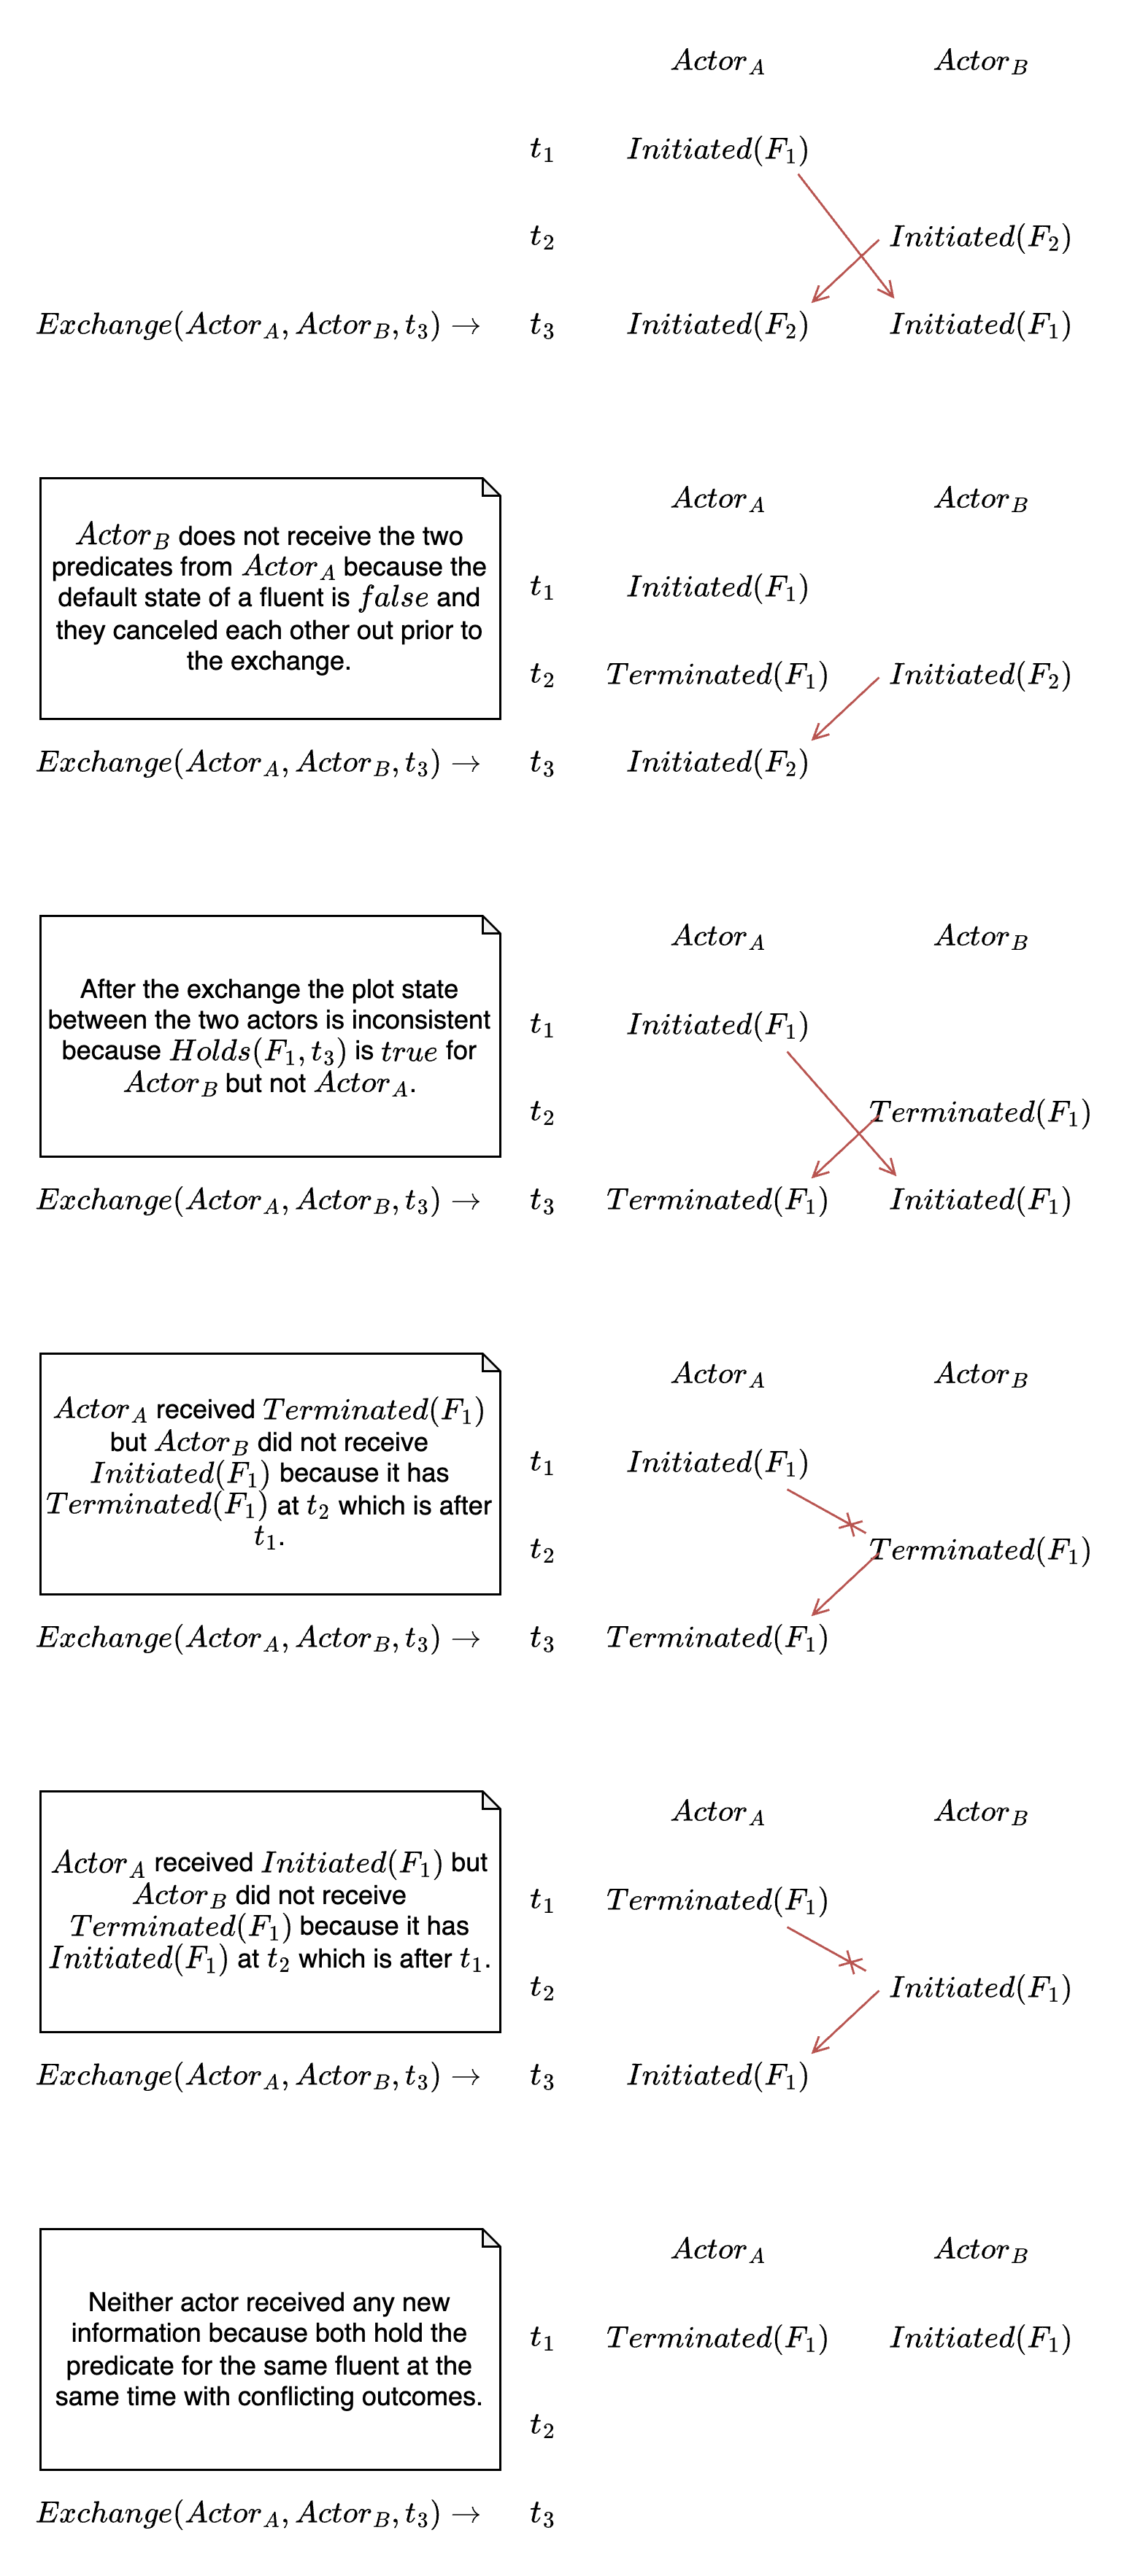
\includegraphics[width=0.55\textwidth]{images/temporal_conflicts_in_event_exchange.drawio.png}
    \caption{Selected outcomes of event exchange between two actors with description of possible conflicts}
    \label{fig:temporal_conflicts_in_event_exchange}
\end{figure}

The problems described above matter only in the case of games where there will be two actors exchanging plot state simultaneously.
Not all games have this requirement and those that do not, that is those with unidirectional information exchange mechanisms, will inherently be free from these pitfalls.
Similarly, some games do not require deterministic state of the plot or the ability for an actor to forget information.
In these types of games, event calculus might not be applicable and other solutions should be considered.

\subsection {Inference rules}

The best approach in choosing the framework for representing plot state depends on the type of plot to be represented and the intended game mechanics.
An RPG game where the player can freely interact with the simulated world will have a different set of requirements than a murder mystery game.
The latter may be satisfied with a probabilistic or confidence-based approach and have no need for actions and instead require inference rules.
In such case the player is usually tasked with solving a mystery based on a set of clues.
In a regular game the solution to the mystery is usually predetermined or semi-random but in general singular per game.
Using a confidence or probabilistic approach, the game may accept any solution as long as the probability for it being correct is above a certain defined threshold.
The concepts of fluents may be borrowed from event calculus to represent individual clues.
For example consider the game as previously described.
The goal of the game is to aquire the fluent $IsCulprit \left( Suspect_N \right)$ where $N$ is the number of the suspect that committed the crime.
The clues in the game are $HasWeapon \left( Suspect_N \right)$ and $HasMotive \left( Suspect_N \right)$.

\begin{equation}
    \label{eqn:weapon_motive_inference}
    HasWeapon \left( Suspect_N \right) \land HasMotive \left( Suspect_N \right) \Rightarrow  IsCulprit \left( Suspect_N \right)
\end{equation}

There is one inference rule defined in equation \ref{eqn:weapon_motive_inference}.
Consider the state of the game where there are three actors $Suspect_A$, $Suspect_B$, $Suspect_C$.
The player can hold a conversation with each of them.
Each conversation yields different clues.

\begin{equation}
    Suspect_A \rightarrow HasWeapon \left( Suspect_B \right) \land HasMotive \left( Suspect_C \right)
\end{equation}

\begin{equation}
    Suspect_B \rightarrow HasMotive \left( Suspect_C \right) \land HasWeapon \left( Suspect_A \right)
\end{equation}

\begin{equation}
    Suspect_C \rightarrow HasMotive \left( Suspect_B \right)
\end{equation}

Based on the inference rule defined for $IsCulprit$ one can get:

\begin{equation}
    HasWeapon \left( Suspect_B \right) \land HasMotive \left( Suspect_B \right) \Rightarrow  IsCulprit \left( Suspect_B \right)
\end{equation}

This is fine until $Suspect_C$ divulges that $HasMotive \left( Suspect_A \right)$.
After this the following holds:

\begin{equation}
    IsCulprit \left( Suspect_A \right) \land IsCulprit \left( Suspect_B \right)
\end{equation}

\subsection{Confidence/probability based inference}

Under the assumption that there is exactly a single culprit, the probabilistic approach can be taken.
Probability function $P(X)$ can be defined for each fluent.

\begin{equation}
    \label{eqn:is_culprit_probability_pre}
    P \left( IsCulprit \left( Suspect_A \right) \right) + P \left( IsCulprit \left( Suspect_B \right) \right) + P \left( IsCulprit \left( Suspect_C \right) \right) = 1
\end{equation}

Because there is no way to attain $IsCulprit \left( Suspect_C \right)$, its probability will be equal to zero and so \ref{eqn:is_culprit_probability_pre} becomes \ref{eqn:is_culprit_probability_post}.

\begin{equation}
    \label{eqn:is_culprit_probability_post}
    P \left( IsCulprit \left( Suspect_A \right) \right) + P \left( IsCulprit \left( Suspect_B \right) \right) = 1
\end{equation}

So far however each outcome is equally probable and there is no way to determine the probability of any suspect being the culprit based on the clues themselves.

% 4. Compare methods
% 5. Present conclusions

% Plot events: 
% Śmierć władcy rozprzestrzeni się od punktu centralnego wzdłuż dróg
% Wybuch wulkanu rozprzetrzeni się od każdego miejsca z którego był widoczny
% Smok będzie widziany na całej jego trasie lotu, uwzględniając czas.
% Epidemia, każdy nowy chory ma większy priorytet

% \section{Partitioning of actors to form spatial models}

% Spatial models can be constructed by partitioning a logical model after assigning each actor its physical location and calculating bounds of each logical network.
% This method requires that actors form disjoint sets of information networks.
% Any plot even propagated to each spatial region can be either made immedietely accessible to all members of the embedded logical model or to a specific subset of actors.
% Similarly an actor may be designated a gateway out of the logical model into the spatial one and gain the ability to propagate information to other spatial regions.
% This way a game world may employ both types of models to essentially store the whole plot state and simulate in detail only the subset of regions that the player is in close proximity to.
% This approach makes usage of the logical model a viable solution for large scale open world games.

% \section{Difference between knowledge and information}

% % What is information?
% The most important distinction when building information propagation models is the one that differentiates knowledge from information.
% The latter can be propagated while the former cannot.
% This is due to the fact that information represents a statement of fact, irrespective of whether it is true or not.
% A claim that people with axes are walking down the road towards the forest can be an information.
% It should be considered to be fundamentally literal and represent nothing more than the messaging mechanism used to convey it.

% % Knowledge
% A person has a mind capable of linking events, seeing connections between facts, identifying patterns and inferring new knowledge from received information.
% Anyone can easily see that such a group of aforementioned people can represent lumberjacks aiming to chop down the trees.
% Note that neither the word lumberjack or the act of chopping down any tree was mentioned before.
% This shows the distinction between what is pure information and what can be considered knowledge.
% After all, how does one come to the conclusion that axes and trees must mean lumberjacks?
% One needs to be aware of the concept of an axe and its function as well as the existence of the trade of forestry to make that connection.

% % Propagation
% After realizing the meaning of people with axes going towards a forest, one can decide to tell others of this news by formulating a new statement of fact: "Lumberjacks are going to the forest".
% A more natural example would be a person telling a friend that someone told them about a group of lumberjacks heading to a forest.
% This is an example of information propagation.
% It can be illustrated more clearly by assuming the person who heard about the people heading towards the forest had recently seen a pack of wolves in the area.
% They might get alarmed and wish to warn the unsuspecting workers.
% The information "there are wolves in the forest" has the characteristic of urgency as well as importance.
% It is urgent because telling it after the workers get to the forest misses the whole point of warning them.
% It is important because it influences their safety.
% These two factors lay the foundation for best possible propagation effect.
% One would immedietely embark on a trip to warn the lumberjacks of the dangers lurking in the forest and probably mention the situation to anyone they pass by.
% This particular situation also has the characteristic of being targeted towards a specific group.

% % TODO: Find characteristics of information in literature
% % Information characteristics
% Information can be urgent, important and have a target group of receiving people.
% Urgency determines the temporal aspect of propagation.
% Importance influences how much effort one is willing to spend delivering the information.
% A target audience limits the list of potential receivers.
% An information can be urgent and not important, that would simply mean that it will expire after some limited time but if the effort to deliver it on time is too great, it is possible that it won't be done.
% It can be important but not urgent just as well.
% In this case it means that it must be delivered but there are no consequences to doing so later rather than sooner.
% It is worth noting however that importance also influences the temporal element of information propagation as more important messages are going to be propagated faster.
% A target audience can be homogeneus (a group of lumberjacks) or have a variety of different people.
% A person doing the propagation can have a list of intended recipents of a message they are carrying.
% There can also be people who are subscribers of selected kinds of information.
% A mother would like to know if anything happens to her child and as such one can say she subscribes information regarding the health of her children.
% In real life there are many more aspects and characteristcs that are deeper and more nuanced that what was described.
% No artifical model can represent accurately the intricacies of the human mind, much less a group of minds.

% % How information and knowledge interact
% Information cannot exist without someone to perceive it and knowledge cannot exist without information.
% Whenever there is some entity that is able to receive information and understand it, it can produce knowledge.
% Information nececessitates a receiver to exist somewhere in the system that can produce knowledge.
% This means that all three must always be present.
% Collections of actors able to receive information and process it into knowledge as well as create new information and share it with other actors will be henceforth reffered to as information systems.

% % Complexity of information systems
% An information system is a set of actors possessing knowledge and wishing to spread it in the form of information.
% Because the complexity of real information systems is too great, simplification needs to be made in order to focus on the important aspects of such a system.
% The key elements of any information system can be identified:
% \begin{itemize}
%     \item Actor - a person capable of processing information, holds knowledge and can produce new information
%     \item Information - statement originating from any information source, ie. an actor
%     \item Information source - any source of information, can be an actor or an inanimate source such as a recording or text
%     \item Information pathway - any link between actors through which information can travel, can affect the information causing distortion or impact the propagation
% \end{itemize}
% Actors may be offered information or they might produce information themselves.
% This must always happen through an information pathway.
% Inanimate sources of information, ie a written book, may exist within the same system and are considered to be always producing some (usually constant) information.
% An actor may react differently when offered different kinds of information or even the same one repeatedly.
% To illustrate that one can imagine being interested in buying a new pair of shoes if seeing the advertisment of them for the first time and getting more annoyed each consecutive time the same advertisment is played.
% % TODO: Cite the work modelling marketing strategy effectiveness
% This behaviour is usually the target of marketing strategy analysis as simply increasing the intensiveness of advertisment broadcast will not increase the demand for the shown product.
% Aside from being able to receive information, an actor may decide to share it with other actors.
% They might decide to choose a target group or broadcast it to everyone they can reach.
% Some actors may seek certain types of information and query for it anytime they can.
% In order to do so, actors must possess some knowledge.

% % Complexity of knowledge
% Knowledge is a set of statements about the world that are consistent (irrespective of truthfulness).
% One can claim that the planet is flat while another person might disagree and it is valid to say that both possess knowledge about the shape of the world.
% A person can then infer new facts on the basis of what they already know and for instance make a claim that travelling past the edge of the Earth will cause the daring explorer to fall to their demise.
% The second person will then receive such information and basing on their opposing set of known statements will reject it and possibly reduce the opinion of the first person, being less likely to believe anything they might then tell them.
% It is however impossible to model the interactions between information necessary to infer new information the same way that happens in the human mind, at the very least not in any feasible way.
% The complexity of interconnectedness of knowledge and information alike is too great to be represented fully.
% One can however make assumptions and put constraints on the type of statements allowed and the knowledge that can be gained and thus create a simplistic representation of an information system.

% % Scope - logical vs spatial
% There are two main types of information systems that can be used to model information propagation:
% % TODO: Add some citation to "podział przestrzeni na abstrakcyjną i fizyczną"
% \begin{itemize}
%     \item spatial - they model information spread across space, usually partitioned into homogeneus segments or tiles
%     \item logical - representing connections between actors without taking into account physical relationships between them
% \end{itemize}
% The first kind of information system, spatial information systems (SIS) can be used to model large scale events happening across the world.
% The most important assumption in these kind of systems is the homogenuity of any given unit of space as defined by the chosen partitioning method.
% They assume that information has some kind of physical propagation characteristic that allows it to travel across space.
% In these systems an actor needs not to be represented individually but rather can be treated as part of a homogeneus group.
% This model might be used to represent how news regarding the death of a ruler might spread from the captial to the most remote villages.
% The second type of information systems, logical information systerms (LIS) work on the basis of individual actors and interactions between them.
% They are ill suited for large scale modelling as the number of actors to be considered would grow considerably.
% Of course, a spatial system can be represented as a logical system if some of the more important regions of the spatial model are chosen and represented as actors in the logical model.

% % What does it mean for information to be considered as propagated?
% The process of propagating information from one actor to another can be considered in the scope of physical information receival as well as logical aspect of interpretation.
% The act of knowledge assimilation is inherently present in the process of actor receiving information from any external source.
% % Is it sufficient to transfer information from source to target?
% Information can reach its target in a plethora of ways.
% In many models
% % What happens after information reaches the target?
% % What are the sources of information?



